\documentclass{beamer}

\title{Practical Bounded Min Registers}
\author{Jordan}
\usepackage{comment}
\usepackage{indentfirst}
\usepackage{amsthm}
\usepackage{amssymb}
\usepackage{amsmath}
\usepackage{mathtools}

%Ceil and Floor
\DeclarePairedDelimiter\ceil{\lceil}{\rceil}
\DeclarePairedDelimiter\floor{\lfloor}{\rfloor}
%Theorem types, use name numbering scheme as the lemma section type.
%\newtheorem{lemma}{Lemma}
%\newtheorem{theorem}[lemma]{Theorem}
%\newtheorem{invariant}[lemma]{Invariant}
%\newtheorem{corollary}[lemma]{Corollary}
%\newtheorem{definition}[lemma]{Definition}
%\newtheorem{assumption}[lemma]{Assumption}
%\newtheorem{mathProof}[lemma]{Supplementary Proof}
\usepackage{hyperref}
%For diagrams.
\usepackage{tikz}
\usepackage{float}
\usetikzlibrary{shapes.geometric}
\usetikzlibrary{positioning}
\usetikzlibrary{graphs}
\usetikzlibrary{matrix}
\usetikzlibrary{decorations.pathreplacing}


%Using this so that I don't have to always reference the name of a theorem
\usepackage{theoremref}
\usepackage{listings}
\usepackage{xcolor}
\usepackage{ulem}
%\usepackage{showlabels}
%Show the labels of theorems
%\showlabels{thlabel}
\usepackage{longtable}
\usepackage{subcaption}
%\usepackage{geometry}
%\geometry{letterpaper}
\renewcommand{\qedsymbol}{}


\definecolor{codegreen}{rgb}{0,0.6,0}
\definecolor{codegray}{rgb}{0.5,0.5,0.5}
\definecolor{codepurple}{rgb}{0.58,0,0.82}
\definecolor{backcolour}{rgb}{0.95,0.95,0.92}
\lstdefinestyle{mystyle}{
	backgroundcolor=\color{backcolour},
	commentstyle=\color{codegreen},
	keywordstyle=\color{magenta},
	numberstyle=\tiny\color{codegray},
	stringstyle=\color{codepurple},
	basicstyle=\ttfamily\footnotesize,
	breakatwhitespace=false,
	breaklines=true,
	captionpos=b,
	keepspaces=true,
	numbers=left,
	escapeinside={@}{@}, %Used for referencing lines in algorithm					
	numbersep=5pt,
	showspaces=false,
	showstringspaces=false,
	showtabs=false,
	morekeywords={},
	tabsize=4,
	emph={},
	emphstyle={\color{blue}}
}
\lstset{style=mystyle}

%Tikz node, edge styles.
\tikzset{vertex/.style = {circle,draw=black, scale=0.7}}
\tikzset{edge/.style = {->, thick}}
\tikzset{dottedEdge/.style = {->,thin,dotted}}
\tikzset{dottedVertex/.style = {circle,draw=black,dotted}}
\tikzset{subtree/.style = {isosceles triangle, text width=4em, draw=black, shape border rotate=90, align=center, anchor=north}}


\newcommand{\twoField}[2]{{\langle}{#1},{#2}{\rangle}}

\usetheme{Copenhagen}
\setbeamertemplate{theorems}[ams style]
\begin{document}
\frame{\titlepage}

\begin{frame}
\frametitle{$b$-bounded min register}
	A $b$-bounded min register is a shared object with initial value $b$, supporting the $minRead()$ and $minWrite(v)$ operations:
	\begin{itemize}
		\item $minRead()$: 
		\begin{itemize}
			\item Return the current value of the register.
		\end{itemize}
		\item $minWrite(v)$, $0 \le v \le b$ 
		\begin{itemize}
			\item If $v$ is less than the current value of the register, write $v$ to the register. 
			\item Otherwise do nothing.
		\end{itemize}
	\end{itemize}
\end{frame}
\begin{frame}
\frametitle{Implementation}
	Based on the Max Register implementation by Aspnes, Attiya and Censor in their paper \textit{Max Registers, Counters, and Monotone Circuits}
	\\~\
	\\~\
	$0$-bounded min register $z$:
	\begin{itemize}
		\item $z.minRead():$
			\begin{itemize}
				\item Return 0
			\end{itemize} 
		\item $z.minWrite(v):$
			\begin{itemize}
				\item Do nothing.
			\end{itemize}
	\end{itemize}
\end{frame}
\begin{frame}
	\begin{lemma}
		$z$ is wait-free and linearizable.
	\end{lemma}
	\begin{lemma}
		The $minWrite$ function is a no-op and the $minRead$ function returns after one instruction.
		For every execution an operation on $z$ is linearized immediately upon the step it is invoked - 
		since $z$ already has value 0 in the initial configuration, the $minWrite$ function, by definition, has no effect.
		The $minRead$ function always returns 0 which is consistent with the state of the object when 
		the $minRead$ was invoked -- $z$ has value 0 throughout the execution.
	\end{lemma}
\end{frame}
\begin{frame}
\frametitle{Implementation}
	Suppose we have a $left.size$-bounded min register $left$, a $right.size$ bounded min register $right$, 
	and a one bit multi-writer register $sw$ with initial value $1$,
	where $0 \le right.size \le left.size$.
	\\~\
	\\~\
	\noindent $(left.size + right.size + 1)$-bounded min register $r$:

	$r.minRead():$
			\begin{itemize}
				\item if $sw = 1$, return $right.minRead()$ + $left.size$ + 1 
				\item else return $left.minRead()$
			\end{itemize} 
		$r.minWrite(v)$:
			\begin{itemize}
				\item if $v > left.size$
				\begin{itemize}
					\item if $sw = 1$, $right.minWrite(v - left.size - 1)$
				\end{itemize}
				\item else
				\begin{itemize}
					\item $left.minWrite(v)$
					\item $sw \leftarrow 0$
				\end{itemize}
			\end{itemize}
\end{frame}
\begin{frame}
	\begin{lemma}
	Suppose $left$ and $right$ are wait-free bounded min registers. Then so is $r$.
	\end{lemma}
	\begin{proof}
		The $r.minRead()$ and $r.minWrite()$ functions use only use a single step to either read or write to $sw$, in addition to using 
		the $minRead()$ and $minWrite()$ functions of $left$ and $right$. 
	\end{proof}
\end{frame}
\begin{frame}
	\begin{lemma}
		Suppose $left$ and $right$ are linearizable bounded min registers. Then so is $r$.
	\end{lemma}
	\begin{proof}
		Consider an execution in which every instance of $r.minRead()$ and $r.minWrite(v)$ instance
		is allowed to complete. Given an incomplete execution $e$, since $r$ is wait-free, we can
		append an extension to allow incomplete instances to finish.

		\begin{itemize}
		\item Let $C_{right}$ be the set of $r.readMin()$ instances that read 1 from $sw$ and 
		$r.writeMin(v)$ ops that read 1 from $sw$ where $v > left.size$.
		\item Let $C_{left}$ be the set of $r.readMin()$ instances that read 0 from $sw$ and 
		$r.writeMin{v}$ ops with $v \le left.size$, and thus write $0$ to $sw$. 
		\item Let $C_{switch}$ be the set of $r.writeMin(v)$ that read 0 from $sw$ where $v > left.size$.
		\end{itemize}
	\end{proof}
\end{frame}

\begin{frame}
	\begin{proof}
		Observe that $C_{left}$ is exactly the set of instances that access $left$. 
		A $r.writeMin(v)$ instance in $C_{left}$ is linearized at the first instant $sw$ is 0 
		after is linearization point on its $left.writeMin(v)$, in the order these operations were linearized.
		\\~\
		In particular, every instance in $C_{switch}$ linearizes after the first such $r.writeMin(v)$
		instance in $C_{left}$ writes 0 to $sw$.  
		And thus these writes in $C_{switch}$ do nothing, since they linearize when $r$
		is already less than or equal to $left.size$.
		\\~\
		A $r.readMin()$ instance in $C_{left}$ is linearized at the same instant 
		that its $left.readMin()$ instance is linearized, before which it reads 0 from $sw$.
		Thus it linearizes after the first instance of $r.writeMin(v)$ in $C_{left}$ has linearized.
	\end{proof}
\end{frame}
\begin{frame}
	\begin{proof}
		Observe that $C_{right}$ is exactly the set of instances that access $right$.
		Every instance in $C_{right}$ is linearized in the same order as the order for their accesses to $right$,
		in either the configuration their access to right takes place or in the configuration before 0 is written to $sw$.
		Since every instance in $C_{right}$ reads 1 from $sw$, their linearization point lies within their operation
		and before any operation in $C_{left}$.
	\end{proof}
\end{frame}
 \begin{frame}
\frametitle{Linearizability proof}
	\begin{figure}
		\centering
		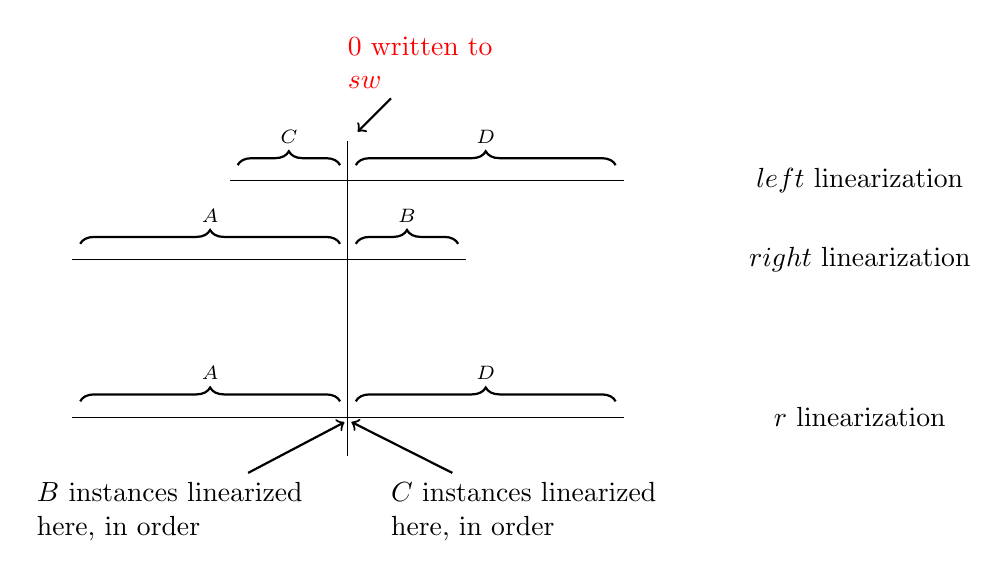
\begin{tikzpicture}[]
		%draw horizontal line
		\node(A) at (3.5,0.5){};
		\node[text width=2cm, color=red](B) at (4.5,1.5){0 written to $sw$};
		\draw[edge] (B) to (A);

		\draw (2,0) -- (3.5,0) -- (7,0); \node at (10,0){$left$ linearization};
		\draw (0,-1) -- (3.5,-1) -- (5.0,-1); \node at(10,-1){$right$ linearization};
		\draw (0,-3) -- (7,-3); \node at (10,-3){$r$ linearization};

		%draw vertical line to represent the write of 0 to sw
		\draw (3.5,0.5) -- (3.5,-3.5);
		\draw [thick ,decorate,decoration={brace,amplitude=5pt}] (2.1,0.2)  -- +(1.3,0) 
		node [black,midway,above=4pt, font=\scriptsize] {$C$};
		\draw [thick ,decorate,decoration={brace,amplitude=5pt}] (3.6,0.2)  -- +(3.3,0) 
		node [black,midway,above=4pt, font=\scriptsize] {$D$};
		\draw [thick ,decorate,decoration={brace,amplitude=5pt}] (0.1,-0.8)  -- +(3.3,0) 
		node [black,midway,above=4pt, font=\scriptsize] {$A$};
		\draw [thick ,decorate,decoration={brace,amplitude=5pt}] (3.6,-0.8)  -- +(1.3,0) 
		node [black,midway,above=4pt, font=\scriptsize] {$B$};
	   
		\draw [thick ,decorate,decoration={brace,amplitude=5pt}] (3.6,-2.8)  -- +(3.3,0) 
		node [black,midway,above=4pt, font=\scriptsize] {$D$};
		\draw [thick ,decorate,decoration={brace,amplitude=5pt}] (0.1,-2.8)  -- +(3.3,0) 
		node [black,midway,above=4pt, font=\scriptsize] {$A$};

		\node(C) at (3.58,-3.0){};
		\node[text width=3.5cm](D) at (1.3,-4.2){$B$ instances linearized here, in order};
		\draw[edge] (D) -- (C);
		\node(E) at (3.42,-3.0){};
		\node[text width=3.5cm](F) at (5.8,-4.2){$C$ instances linearized here, in order};
		\draw[edge] (F) -- (E);
		%draw vertical lines
		%\foreach \x in {0,2,5,7}{\draw (\x,3pt) -- (\x,-3pt);}
		%Draw nodes
		%\draw (0,0) node[above=3pt, text width = 3cm] { $w_{i+1}$ performs $R.update()$ } node[below=3pt] {(1)};
		%\draw (2,0) node[above=3pt, text width = 1.5cm] {$w_{i+x+1}$ finishes} node[below=3pt] {(2)};
		%\draw (5,0) node[above=3pt, text width = 3cm] { $w_i$ performs $R.update()$  } node[below=3pt] {(3)};
		%\draw (7,0) node[above=3pt, xshift=1cm,  text width = 3cm, color = red] {$w_{i+1}$ performs $R.update()$} node[below=3pt, color = red] {(1)};
		\end{tikzpicture}
		%\caption{}
	\end{figure}
\end{frame}
   
\begin{frame}
\frametitle{Practical Implementations of a $b$-bounded min register}
Idea 1: A $b$-bounded min register object stores fields $sw$ (the multiwriter bit register), $size$ (equal to $b$), 
and $left$, $right$ which are pointers to $\ceil{\frac{b-1}{2}}$ and $\floor{\frac{b-1}{2}}$-bounded min register objects respectively.
\\
Pros:
\begin{itemize}
	\item Very simple to implement.
	\item Might reduce contention to store objects at different places in memory
\end{itemize}
Cons
\begin{itemize}
	\item A lot of wasted space. On 64 bit systems, at least 24 bytes per node used, so total space used is $24b$ bytes.
	\begin{itemize}
		\item Jeremy's trie, with height = $b$ requires a $b+1$ bounded min register for every DelNode
		\item A trie of height = 31 has $2^{30}$ delete nodes initially, thus this would be 500gb for the min registers alone!
	\end{itemize}
	\item Slow to traverse to different bounded min register objects from $left/right$.
\end{itemize}
\end{frame}
\begin{frame}
\frametitle{Practical Implementations of a $b$-bounded min register}
Idea 2: We can use an array-based tree, with where each array element (node) stores a switch register.
\end{frame}
\begin{frame}[fragile]
\frametitle{Array-based leveled binary tree}
\begin{definition}
	A binary tree is leveled if every row, except possibly the last is filled.
\end{definition}
We can use a $b$-element array of atomic registers as a $b$ node leveled binary tree. 
In a leveled binary tree, the left child (if it exists) of a node at index $i$ is at index $2i + 1$, and the right child (if it exists) is at index $2i + 2$.
\begin{figure}
	\begin{subfigure}[b]{0.47\textwidth}
	\centering
	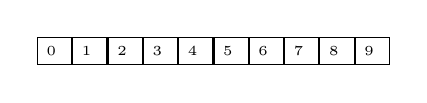
\begin{tikzpicture}
		\matrix [nodes={rectangle, draw=black, text width=2mm,anchor=west, font=\tiny }]
		{
			\node{0}; & \node{1}; & \node{2}; & \node{3}; & \node{4}; & \node{5}; & \node{6}; & \node{7}; & \node{8}; & \node{9}; \\
		};
	\end{tikzpicture}
	\hspace{10cm}
	\end{subfigure}
\hfill
	\begin{subfigure}[b]{0.47\textwidth}
	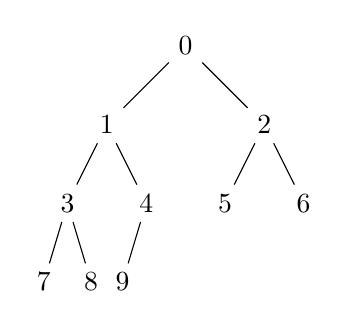
\begin{tikzpicture}
		\node(A) at (0,0){0};

		\node(B) at (-1,-1){1};
		\node(C) at (1,-1){2};

		\node(D) at (-1.5,-2){3};
		\node(E) at (-0.5,-2){4};
		\node(F) at (0.5,-2){5};
		\node(G) at (1.5,-2){6};

		\node(H) at (-1.8,-3){7};
		\node(I) at (-1.2,-3){8};
		\node(J) at (-0.8,-3){9};

		\draw (A) -- (B) -- (D) -- (H);
		\draw (A) -- (C) -- (G);
		\draw (D) -- (I);
		\draw (C) -- (F);
		\draw (B) -- (E) -- (J);
	\end{tikzpicture}
	\end{subfigure}
\end{figure}
\end{frame}
\begin{frame}
%size formula from integer sequences website....
The number of nodes in the left subtree in a leveled binary tree of size $n$:
\begin{align*}
	a(n) = He(n) \cdot (n + 2^{\floor{\log_2(n)}-1} - 1) + (-1)^{He(n)}\cdot(2^{\floor{\log_2(n)}} - 1)
\end{align*}
where 
\begin{align*}
	He(n) = H(-n + 3\cdot2^{\floor{\log_2(n)}-1} - 1) 
\end{align*}
and 
\begin{align*}
	H(x) = [x \ge 0]
\end{align*}
Proof by Bozinovski available here.
https://oeis.org/A279521
\end{frame}
\begin{frame}
Pros:
\begin{itemize}
	\item More cache friendly - on x86-64 machines, accessing a single byte results in loading the next 63 bytes.
	If the cache is not invalidated after accessing first element of array, successive accesses do no incur a cache miss!
\end{itemize}
Cons:
\begin{itemize}
	\item Now need $b$ bytes for a size $b$ register, which is better, but a Trie of height $32$ would require 32 extra bytes per node 
	for the min register alone, which is not great.
	\item If contention is high, cache may be invalidated by other threads that modify even different parts of the array, causing 
	cache misses on successive reads/writes. (False sharing)
\end{itemize}
\end{frame}
\begin{frame}[fragile]
\frametitle{But wait, there's more!}
We are only using 1 bit for every byte in the array...
What if instead we could use \emph{every bit} in the array rather than one per byte?
8 times the capacity!
\begin{itemize}
\item Before:
\\
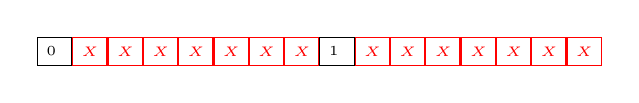
\begin{tikzpicture}
	\matrix [nodes={rectangle, draw=black, text width=2mm,anchor=west, font=\tiny }]
	{
		\node{0}; & \node[color=red]{$X$}; & \node[color=red]{$X$}; & \node[color=red]{$X$}; & \node[color=red]{$X$}; & \node[color=red]{$X$}; & \node[color=red]{$X$}; & \node[color=red]{$X$}; &
		\node{1}; & \node[color=red]{$X$}; & \node[color=red]{$X$}; & \node[color=red]{$X$}; & \node[color=red]{$X$}; & \node[color=red]{$X$}; & \node[color=red]{$X$}; & \node[color=red]{$X$}; \\
	};
	
\end{tikzpicture}

\item After:
\\
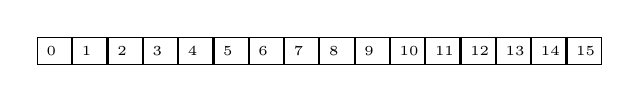
\begin{tikzpicture}
	\matrix [nodes={rectangle, draw=black, text width=2mm,anchor=west, font=\tiny }]
	{
		\node{0}; & \node{1}; & \node{2}; & \node{3}; & \node{4}; & \node{5}; & \node{6}; & \node{7}; &
		\node{8}; & \node{9}; & \node{10}; & \node{11}; & \node{12}; & \node{13}; & \node{14}; & \node{15}; \\
	};
\end{tikzpicture}
\end{itemize}
%bit array diagram
%TODO bit array diagram....
\end{frame}
\begin{frame}[fragile]
\frametitle{Reads and Writes to individual bits}
Reading a particular bit atomically is trivial...
But what about writing 0 to particular bit? 
There's an atomic operation for that, we can use $fetch\&and$!

To write 0 to bit $i$ of a particular byte $a$ atomically, we can use $fetch\&and(address(a), 11111111_2 - (1 << (7 - i)))$ 

For example to write 0 to bit 4 of a byte $x = 01001100_2$, we can use $fetch\&and(\&x,11110111_2)$, which will turn off bit 4 and leave the other bits unchanged.
\end{frame}
\begin{frame}
	\frametitle{Implementation for $Jeremy$'s trie}
	If we restrict the maximum size of the register to $2^k - 1$ for some $k$, 
	then the size of the left subtree = size of right subtree = $\floor{\frac{2^k-1}{2}}$.
	\\~\
	I have reimplemented the $minWrite$ and $minRead$ functions to be iterative, 
	and I use a 63-bounded min register using an array of 8 bytes.
	Initially the min register has value 63 but can be initialized to $b$ with the use of
	$minWrite(b)$.
\end{frame}
\begin{frame}
	\frametitle{Consequences}
	Pros:
	\begin{itemize}
		\item Can use use 8 bytes for a 63 bit bounded min register, rather than 63 bytes.
		\item No more risk of false sharing than with the array implementation.
	\end{itemize}
	Cons
	\begin{itemize}
		\item Contention costs may be higher since more registers are stored within the same byte.
		\item Doing a lot of reads from/writes to shared memory since we only read or write one bit at a time
	\end{itemize}
\end{frame}
\begin{frame}
	\frametitle{One more thing}
	Notice that any reads occur before any writes in both minRead and minWrite operations.
	
	Reads will read switches before going down the tree.
	Writes will read switches before going down the tree, then write on their way back up the tree.

	There's no need for a gap between any two successive reads -- or any two successive $fetch\&and$s!
	Why not do all reads at the same time, and all $fetch\&ands$ at the same time!
	Then reads only need to read one 8 byte integer from memory, 
	and writes only need to read one 8 byte integer from memory, then $fetch\&and$ one.
\end{frame}

\end{document}
